\documentclass[12pt]{article}
\usepackage[margin=1in]{geometry}
\usepackage{amsmath, amssymb, amsthm, graphicx, hyperref}
\usepackage{amsmath}
\usepackage{enumerate}
\usepackage{fancyhdr}
\usepackage{multirow, multicol}
\usepackage{tikz}
\usepackage{wrapfig}
\pagestyle{fancy}
\usepackage{titlesec}
\usepackage{lastpage}
\usepackage{multirow}
\usepackage{indentfirst}
\fancyhead[LO]{JACK Z}
\fancyhead[RO]{Page \thepage\ of \pageref{LastPage}}
\usepackage{comment}
\newtheorem{definition}{Definition}
\usepackage{amsmath}
\usepackage{booktabs}
\usepackage{xcolor}
\usepackage{tcolorbox}  % For creating styled boxes
\tcbuselibrary{most}
\usepackage{tcolorbox} % for creating colored or framed text boxes
\tcbuselibrary{breakable} % allows tcolorboxes to break across pages

\definecolor{examplebg}{RGB}{255, 228, 225} % Light red background
\tcbuselibrary{theorems} 
\usepackage{graphicx}
\usepackage{booktabs} % For better table formatting
\usepackage{caption} % Essential for \captionof
\usepackage{tcolorbox} % For creating colored boxes
\tcbuselibrary{most} % Load most libraries for tcolorbox



\newtcbtheorem[number within=subsection]{Definition}{Definition}{
    colback=blue!5,
    colframe=blue!35!black,
    fonttitle=\bfseries,
    colbacktitle=blue!85!black,
    coltitle=white,
    enhanced,
    attach boxed title to top left={yshift=-2mm, xshift=2mm},
    boxed title style={sharp corners},
    sharp corners
}{def}

\newtcbtheorem[number within=subsection]{mytheorem}{Theorem}{
    colback=orange!5,      % Background color of the box
    colframe=orange,     % Border color of the box
    coltitle=white,     % Color of theorem title
    colbacktitle=orange!85!black,, % Background color for the title
    fonttitle=\bfseries,
    title after break={Theorem \csname the\tcbcounter\endcsname\ -- Continued}, % for continued theorems
    enhanced,
    attach boxed title to top left={yshift=-2mm, xshift=2mm},
    boxed title style={sharp corners, colframe=black},
    sharp corners,
    separator sign none % no sign between title and theorem text
}{thm}


\usepackage{lipsum} % 生成示例文本
\usepackage{fancyhdr}

\pagestyle{fancy}
\renewcommand{\headrulewidth}{0pt} % 去掉页眉下方的横线
\fancyfoot[C]{\textcopyright\ \fcolorbox{purple}{white}{Novel Prep}}

% Define custom colors
\definecolor{deepblue}{rgb}{0.0, 0.18, 0.39}
\definecolor{deepred}{rgb}{0.6, 0, 0}

% Define theorem style
\newtheoremstyle{beautifulthm}
  {10pt} % Space above
  {10pt} % Space below
  {\itshape} % Body font
  {} % Indent amount
  {\bfseries\color{deepblue}} % Theorem head font
  {.} % Punctuation after theorem head
  {.5em} % Space after theorem head
  {} % Theorem head spec

\theoremstyle{beautifulthm}
\newtheorem{theorem}{Theorem}[section]
\begin{document}

\title{AP Calculus AB\&BC}
\author{Hongjun Zeng}
\maketitle

\lipsum[1-10] 

\newpage
\tableofcontents

\newpage
\section{Limits and Continuity}
\subsection{Finding Limits Graphically and Numerically}
\subsubsection*{An Introduction to Limits}

The limit of a function describes the value that a function approaches as the input approaches some value.


\begin{Definition}{}{}
Let \( f \) be a function defined on an open interval that contains the point \( c \), except possibly at \( c \) itself. We say that the limit of \( f \) as \( x \) approaches \( c \) is \( L \), and we write:
\[
\lim_{x \to c} f(x) = L
\]
if for every number \( \epsilon > 0 \) there exists a number \( \delta > 0 \) such that if \( 0 < |x - c| < \delta \), then \( |f(x) - L| < \epsilon \).
\end{Definition}

\begin{tcolorbox}[colback=examplebg, colframe=red!75!black, title=\textbf{EXAMPLE 1: Estimating a Limit Numerically}, fonttitle=\bfseries, sharp corners]
\textbf{Evaluate the function} \( f(x) = \frac{x}{\sqrt{x + 1} - 1} \) \textbf{at several \( x \)-values near 0 and use the results to estimate the limit}

\[
\lim_{x \to 0} \frac{x}{\sqrt{x + 1} - 1}
\]

\tcblower
\subsection*{Solution}
The table lists the values of \( f(x) \) for several \( x \)-values near 0.

\textbf{x approaches 0 (left)} \hspace{3cm} \textbf{x approaches 0 (right)}

\begin{tabular}{cccccccc}
\toprule
\( x \)    & -0.01    & -0.001   & -0.0001  & 0     & 0.0001  & 0.001   & 0.01    \\
\midrule
\( f(x) \) & 1.99499  & 1.99950  & 1.99995  & ?     & 2.00005 & 2.00050 & 2.00499 \\
\bottomrule
\end{tabular}
% Using minipage to include the image non-floating
\begin{minipage}{\linewidth}
    \centering
    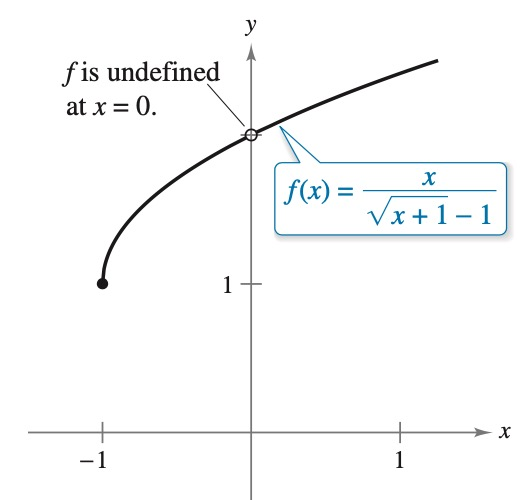
\includegraphics[width=0.37\linewidth]{Example_1.jpg} % Adjust the image width as necessary
    \captionof{figure}{The limit of \( f(x) \) as \( x \) approaches 0 is 2.}
    \label{fig:graph}
\end{minipage}

\end{tcolorbox}

\newpage
\subsubsection*{Limits That Fail to Exist}
 A limit may fail to exist for several reasons, including if the function approaches different values from different directions (left-hand limit and right-hand limit are different),
\begin{tcolorbox}[colback=examplebg, colframe=red!75!black, title=\textbf{EXAMPLE 2: Different Right and Left Behavior}, fonttitle=\bfseries, sharp corners]

\textbf{Show that the limit
\[
\lim_{x \to 0} \frac{|x|}{x}$
\]
does not exist.}
\tcblower
\subsection*{Solution}
Consider the graph of the function
\[
f(x) = \frac{|x|}{x}.
\]
From the definition of absolute value, we know:
\[
|x| = 
\begin{cases} 
x, & \text{if } x \geq 0, \\
-x, & \text{if } x < 0
\end{cases}
\] % End of absolute value definition

This gives us:
\[
\frac{|x|}{x} = 
\begin{cases} 
1, & \text{if } x > 0, \\
-1, & \text{if } x < 0
\end{cases}
\] % End of function definition

Since the limits as \(x\) approaches zero from the right and left are different, the overall limit does not exist. The function approaches 1 from the right and -1 from the left.
\end{tcolorbox}


\newpage

\subsection{Determining Limits Using Algebraic Properties of Limits}
\subsubsection{Some Properties of Limits}
In previous section, you learned that the limit of \( f(x) \) as \( x \) approaches \( c \) does not depend on the value of \( f \) at \( x = c \). It may happen, however, that the limit is precisely \( f(c) \). In such cases, the limit can be evaluated by \textbf{\textit{direct substitution}}. That is,
\[
\lim_{x \to c} f(x) = f(c) \quad \text{\textcolor{red}{Substitute \( c \) for \( x \).}}
\]
Such well-behaved functions are \textbf{continuous at \( c \)}. 
\begin{mytheorem}{Some Basic Limits}{basiclimits}
Let \(b\) and \(c\) be real numbers, and let \(n\) be a positive integer. Then:
\begin{enumerate}
    \item \(\lim_{x \to c} b = b\)
    \item \(\lim_{x \to c} x = c\)
    \item \(\lim_{x \to c} x^n = c^n\)
\end{enumerate}
\end{mytheorem}

\begin{tcolorbox}[colback=examplebg, colframe=red!75!black, title=\textbf{EXAMPLE 1: Evaluating Basic Limits} , fonttitle=\bfseries, sharp corners]
Find the Limit
\textbf{\begin{enumerate}
    \item[a.] 
    \(\lim_{x \to 2} 3 = 3\)
    \item[b.] \(\lim_{x \to -4} x = -4\)
    \item[c.] \(\lim_{x \to 2} x^2 = 2^2 = 4\)
\end{enumerate}}
\end{tcolorbox}
 Limits help us define and analyze these behaviors, providing the foundational concepts necessary for the derivatives and integrals. The properties of limits simplify complex limit evaluations and offer a deeper insight into the continuity and differentiability of functions.
\begin{mytheorem}{Properties of Limits}{propertiesoflimits}
Let \(b\) and \(c\) be real numbers, let \(n\) be a positive integer, and let \(f\) and \(g\) be functions with the limits
\[
\lim_{x \to c} f(x) = L \quad \text{and} \quad \lim_{x \to c} g(x) = K.
\]
\begin{enumerate}
    \item Scalar multiple: \(\lim_{x \to c} [b f(x)] = bL\)
    \item Sum or difference: \(\lim_{x \to c} [f(x) + g(x)] = L + K\)
    \item Product: \(\lim_{x \to c} [f(x) g(x)] = LK\)
    \item Quotient: \(\lim_{x \to c} \frac{f(x)}{g(x)} = \frac{L}{K}\), \(K \neq 0\)
    \item Power: \(\lim_{x \to c} [f(x)]^n = L^n\)
\end{enumerate}
\end{mytheorem}

\begin{tcolorbox}[colback=examplebg, colframe=red!75!black, title=\textbf{EXAMPLE 2: The Limit of a Polynomial}, fonttitle=\bfseries, sharp corners]
Find the limit: 
\[
\(\lim_{x \to 2} (4x^2 + 3)\).
\]
\tcblower
\textbf{Solution} \\
\[
\lim_{x \to 2} (4x^2 + 3) = \lim_{x \to 2} 4x^2 + \lim_{x \to 2} 3
\]
This can be simplified by calculating each limit separately:
\[
= 4 \cdot \lim_{x \to 2} x^2 + 3
\]
Since the limit of a constant is the constant itself and the limit of \(x^2\) as \(x\) approaches 2 is \(4\):
\[
= 4 \cdot 4 + 3 = 16 + 3 = 19
\]
\end{tcolorbox}


\begin{mytheorem}{Properties of Limits}{propertiesoflimits}
\textit{If \( p \) is a polynomial function and \( c \) is a real number, then}
\[
\lim_{x \to c} p(x) = p(c).
\]

\textit{If \( r \) is a rational function given by \( r(x) = \frac{p(x)}{q(x)} \) and \( c \) is a real number such that \( q(c) \neq 0, \) then}
\[
\lim_{x \to c} r(x) = r(c) = \frac{p(c)}{q(c)}.
\]
\end{mytheorem}


\begin{tcolorbox}[colback=examplebg, colframe=red!75!black, title=\textbf{EXAMPLE 3: The Limit of a Rational Function}, fonttitle=\bfseries, sharp corners]
\textbf{Find the limit:} \( \lim_{x \to 1} \frac{x^2 + x + 2}{x + 1} \).
\tcblower
\textbf{Solution} \\
Because the denominator is not 0 when \( x = 1 \), you can apply Theorem 1.2.3 to obtain
\[
\lim_{x \to 1} \frac{x^2 + x + 2}{x + 1} = \frac{1^2 + 1 + 2}{1 + 1} = \frac{4}{2} = 2.
\]
\end{tcolorbox}
The next theorem greatly expands your ability to evaluate limits because it shows how to analyze the limit of a composite function.
\begin{mytheorem}{The Limit of a Composite Function}{propertiesoflimits}
\textit{If \( f \) and \( g \) are functions such that \( \lim_{x \to c} g(x) = L \) and \( \lim_{x \to L} f(x) = f(L) \), then}
\[
\lim_{x \to c} f(g(x)) = f\left(\lim_{x \to c} g(x)\right) = f(L).
\]
\end{mytheorem}

\begin{tcolorbox}[colback=examplebg, colframe=red!75!black, title=\textbf{EXAMPLE 4: The Limit of a Composite Function} fonttitle=\bfseries, sharp corners]
\textbf{Find the limit.}


\begin{enumerate}
    \item[(a)] 
    \[
    \lim_{x \to 0} \sqrt{x^2 + 4}
    \]
    \textbf{Solution} \\

    Because
    \[
    \lim_{x \to 0} (x^2 + 4) = 0^2 + 4 = 4 \quad \text{and} \quad \lim_{x \to 4} \sqrt{x} = \sqrt{4} = 2,
    \]
    you can conclude that
    \[
    \lim_{x \to 0} \sqrt{x^2 + 4} = \sqrt{4} = 2.
    \]

    \item[(b)] 
    \[
    \lim_{x \to 3} \sqrt[3]{2x^2 - 10}
    \]
    \textbf{Solution} \\
    \hrulefill % Adds a horizontal line for visual separation
    \smallskip % Adds a small vertical space for better readability
    Because
    \[
    \lim_{x \to 3} (2x^2 - 10) = 2(3^2) - 10 = 8 \quad \text{and} \quad \lim_{x \to 8} \sqrt[3]{x} = \sqrt[3]{8} = 2,
    \]
    you can conclude that
    \[
    \lim_{x \to 3} \sqrt[3]{2x^2 - 10} = \sqrt[3]{8} = 2.
    \]
\end{enumerate}

\end{tcolorbox}

\noindent \textbf{Note:} The limits of many algebraic functions can be evaluated by direct substitution. This method is particularly useful when the function is continuous at the point of interest.

\subsubsection{A Strategy for Finding Limits}
On 1.3.1, we can use direct substitution to evaluate the Limit. This knowledge, together with the next theorem, can be used to develop a strategy for finding limits

\begin{mytheorem}{Functions That Agree at All but One Point}{propertiesoflimits}
\textbf{}

Let \( c \) be a real number, and let \( f(x) = g(x) \) for all \( x \neq c \) in an open interval containing \( c \). If the limit of \( g(x) \) as \( x \) approaches \( c \) exists, then the limit of \( f(x) \) also exists and
\[
\lim_{x \to c} f(x) = \lim_{x \to c} g(x).
\]
\end{mytheorem}

\begin{tcolorbox}[colback=examplebg, colframe=red!75!black, title=\textbf{EXAMPLE 5: Finding the Limit of a Function},fonttitle=\bfseries, sharp corners]
\textbf{Find the limit.}
\[
\lim_{x \to 1} \frac{x^3 - 1}{x - 1}
\]
\tcblower
\textbf{Solution}

Let \( f(x) = \frac{x^3 - 1}{x - 1} \). By factoring and dividing out like factors, you can rewrite \( f \) as
\[
f(x) = \frac{(x - 1)(x^2 + x + 1)}{x - 1} = x^2 + x + 1 = g(x), \quad x \neq 1.
\]
So, for all \( x \)-values other than \( x = 1 \), the functions \( f \) and \( g \) agree, as shown in Figure 1.17. Because \( \lim_{x \to 1} g(x) \) exists, you can apply Theorem 1.2.5 to conclude that \( f \) and \( g \) have the same limit at \( x = 1 \).

\[
\lim_{x \to 1} \frac{x^3 - 1}{x - 1} = \lim_{x \to 1} (x - 1)(x^2 + x + 1) = \lim_{x \to 1} \frac{(x - 1)(x^2 + x + 1)}{x - 1}
\]
\[
= \lim_{x \to 1} (x^2 + x + 1) = 1^2 + 1 + 1 = 3
\]
% Using minipage to include the image non-floating
\begin{minipage}{\linewidth}
    \centering
    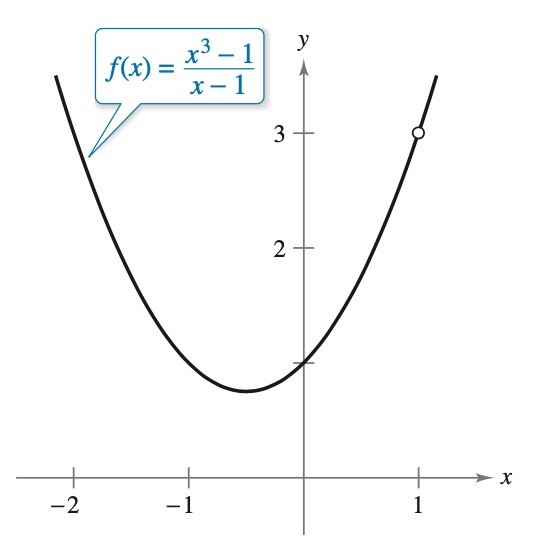
\includegraphics[width=0.37\linewidth]{Example_3.jpg} % Adjust the image width as necessary
    \captionof{figure}{The Function has a hole at x = 1 }
    \label{fig:graph}
\end{minipage}

\end{tcolorbox}


\noindent \textbf{Note:}
\textbf{A Strategy for Finding Limits:}
\begin{enumerate}
    \item Learn to recognize which limits can be evaluated by direct substitution. 
    (These limits are listed in Theorems 1.1 through 1.6.)
    \item When the limit of \( f(x) \) as \( x \) approaches \( c \) cannot be evaluated by direct substitution, try to find a function that agrees with \( f \) for all \( x \) other than \( x = c \). [Choose \( g \) such that the limit of \( g(x) \) \textit{can} be evaluated by direct substitution.] Then apply Theorem 1.7 to conclude \textit{analytically} that
    \[
    \lim_{x \to c} f(x) = \lim_{x \to c} g(x) = g(c).
    \]
    \item Use a graph or table to reinforce your conclusion.
\end{enumerate}

\noindent \textbf{Dividing out technique}

One procedure for finding a limit analytically is the \textbf{dividing out technique} . This technique involves dividing out common factors, as shown in Example 6.
\begin{tcolorbox}[colback=examplebg, colframe=red!75!black, title=\textbf{EXAMPLE 6: Dividing Out Technique}, fonttitle=\bfseries, sharp corners]
\textbf{Find the limit:}
\[
\lim_{x \to -3} \frac{x^2 + x - 6}{x + 3}
\]
\tcblower
\textbf{Solution} \\
Although you are taking the limit of a rational function, you \textit{cannot} apply Theorem 1.3 because the limit of the denominator is 0.

\[
\lim_{x \to -3} (x^2 + x - 6) = 0 \quad \text{and} \quad \lim_{x \to -3} (x + 3) = 0 \quad \text{(Direct substitution fails.)}
\]

Because the limit of the numerator is also 0, the numerator and denominator have a \textit{common factor} of \( (x + 3) \). So, for all \( x \neq -3 \), you can divide out this factor to obtain:

\[
f(x) = \frac{x^2 + x - 6}{x + 3} = \frac{(x+3)(x-2)}{x+3} = x - 2 = g(x), \quad x \neq -3.
\]

Using Theorem 1.5, it follows that:
\[
\lim_{x \to -3} \frac{x^2 + x - 6}{x + 3} = \lim_{x \to -3} (x - 2) = -5.
\]
\begin{minipage}{\linewidth}
    \centering
    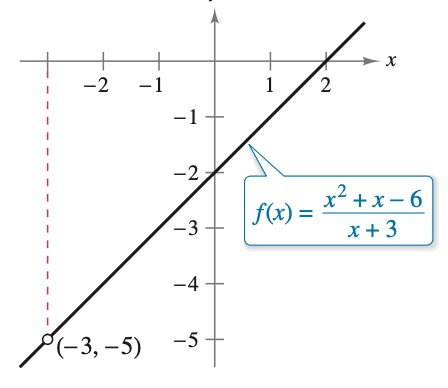
\includegraphics[width=0.37\linewidth]{Example_4.jpg} % Adjust the image width as necessary
    \captionof{figure}{f is not defined at x =  -3 }
    \label{fig:graph}
\end{minipage}
\end{tcolorbox}


\noindent \textbf{Rationalizing Technique}

Another way to find a limit analytically is the \textbf{rationalizing technique}, which involves rationalizing the numerator of a fractional expression.
\begin{tcolorbox}[colback=examplebg, colframe=red!75!black, title=\textbf{EXAMPLE 7: The Limit of a Rational Function}, fonttitle=\bfseries, sharp corners]

\textbf{Find the limit:}
\[
\lim_{x \to 0} \frac{\sqrt{x + 1} - 1}{x}
\]

\tcblower
\textbf{Solution} \\
By direct substitution, you obtain the indeterminate form \(0/0\):
\[
\lim_{x \to 0} (\sqrt{x + 1} - 1) = 0 \quad \text{and} \quad \lim_{x \to 0} x = 0 \quad \text{(Direct substitution fails.)}
\]

In this case, you can rewrite the fraction by rationalizing the numerator:
\[
\frac{\sqrt{x + 1} - 1}{x} = \frac{\sqrt{x + 1} - 1}{x} \cdot \frac{\sqrt{x + 1} + 1}{\sqrt{x + 1} + 1} = \frac{(x + 1) - 1}{x(\sqrt{x + 1} + 1)} = \frac{x}{x(\sqrt{x + 1} + 1)}
\]
\[
= \frac{1}{\sqrt{x + 1} + 1}
\]
Now, using Theorem 1.2.5, you can evaluate the limit as shown:
\[
\lim_{x \to 0} \frac{\sqrt{x + 1} - 1}{x} = \lim_{x \to 0} \frac{1}{\sqrt{x + 1} + 1} = \frac{1}{1 + 1} = \frac{1}{2}
\]

\end{tcolorbox}
\newpage
\noindent \textbf{The Squeeze Theorem}

This method concerns the limit of a function that is \textbf{squeezed} between two other functions, each of which has the same limit at a given x-value
\begin{mytheorem}{Squeeze Theorem}{Squeeze Theorem}

If \( h(x) \leq f(x) \leq g(x) \) for all \( x \) in an open interval containing \( c \), except possibly at \( c \) itself, and if
\[
\lim_{x \to c} h(x) = L = \lim_{x \to c} g(x),
\]
then \( \lim_{x \to c} f(x) \) exists and is equal to \( L \).

\begin{minipage}{\linewidth}
    \centering
    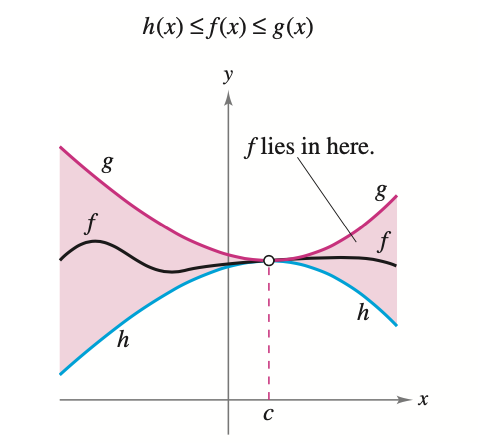
\includegraphics[width=0.37\linewidth]{Example_5.jpg} % Adjust the image width as necessary
    \captionof{figure}{}
    \label{fig:graph}
\end{minipage}
\end{mytheorem}

\begin{tcolorbox}[colback=examplebg, colframe=red!75!black, title=\textbf{EXAMPLE 8: Using the Squeeze Theorem to Find the Limit}, fonttitle=\bfseries, sharp corners]
\textbf{}
\[
\lim_{t \to 0} \left( t^2 \sin \frac{1}{t} \right) = 0
\]
\tcblower
\textbf{Solution} \\
We know that
\[
-1 \leq \sin \frac{1}{t} \leq 1
\]

Multiplying through by \( t^2 \) (which is always non-negative for all real \( t \)) gives:
\[
-t^2 \leq t^2 \sin \frac{1}{t} \leq t^2
\]

Since \(\lim_{t \to 0} (-t^2) = 0\) and \(\lim_{t \to 0} (t^2) = 0\), by the Squeeze Theorem:
\[
\lim_{t \to 0} \left( t^2 \sin \frac{1}{t} \right) = 0
\]
\end{tcolorbox}

\newpage
\noindent\textbf{Two Special Trigonometric Limits}

Here we have two special trigonometric limits that can help you to figure out the Question.

\begin{mytheorem}{Two Special Trigonometric Limits}{Two Special Trigonometric Limits}
\begin{enumerate}
    \item 
    \(\lim_{x \to 0} \frac{\sin x}{x} = 1\)
    
    \item \(\lim_{x \to 0} \frac{1 - \cos x}{x} = 0\)
\end{enumerate}
\end{mytheorem}

\begin{tcolorbox}[colback=examplebg, colframe=red!75!black, title=\textbf{EXAMPLE 9: The Limit of a Rational Function}, fonttitle=\bfseries, sharp corners]
\textbf{Find the limit:}
\[
\lim_{x \to 0} \frac{\sin 4x}{x}
\]
\tcblower
\textbf{Solution} \\
Direct substitution yields the indeterminate form \( \frac{0}{0} \). To solve this problem, you can rewrite the limit as:
\[
\lim_{x \to 0} \frac{\sin 4x}{x} = 4 \left( \lim_{x \to 0} \frac{\sin 4x}{4x} \right) \quad \text{(Multiply and divide by 4.)}
\]
Now, by letting \( y = 4x \) and observing that \( x \) approaches 0 if and only if \( y \) approaches 0, you can write:
\[
\lim_{x \to 0} \frac{\sin 4x}{x} = 4 \left( \lim_{y \to 0} \frac{\sin y}{y} \right) \quad \text{(Let \( y = 4x \).)}
\]
Applying Theorem 1.2.7 (1), which states \( \lim_{y \to 0} \sin y / y = 1 \):
\[
= 4(1) = 4.
\]
\end{tcolorbox}







\newpage

\subsection{Continuity and One-Sided Limits}
\begin{Definition}{ Continuity}{}
\textbf{Continuity at a Point}\\
A function \(f\) is continuous at \(c\) when these three conditions are met:
\begin{enumerate}
    \item \(f(c)\) is defined.
    \item \(\lim_{x \to c} f(x)\) exists.
    \item \(\lim_{x \to c} f(x) = f(c)\).
\end{enumerate}


\end{Definition}

\begin{tcolorbox}[colback=examplebg, colframe=red!75!black, title=\textbf{EXAMPLE 1:Where are each of the following functions discontinuous?}, fonttitle=\bfseries, sharp corners]
\begin{itemize}
    \item[(a)] \( f(x) = \frac{x^2 - x - 2}{x - 2} \)
    \item[(b)] \( f(x) = \begin{cases} 
    \frac{x^2 - x - 2}{x - 2} & \text{if } x \neq 2 \\
    1 & \text{if } x = 2 
    \end{cases} \)
    \item[(c)] \( f(x) = \begin{cases} 
    \frac{1}{x^2} & \text{if } x \neq 0 \\
    1 & \text{if } x = 0 
    \end{cases} \)
    \item[(d)] \( f(x) = |x| \)
\end{itemize}

\tcblower
\textbf{Solution} \\
\begin{itemize}
    \item[(a)] Notice that \( f(2) \) is not defined, so \( f \) is discontinuous at 2. It is continuous at all other numbers.
    \item[(b)] Here \( f(2) = 1 \) is defined and
    \[
    \lim_{x \to 2} f(x) = \lim_{x \to 2} \frac{x^2 - x - 2}{x - 2} = \lim_{x \to 2} (x + 1) = 3.
    \]
    But
    \[
    \lim_{x \to 2} f(x) \neq f(2),
    \]
    so \( f \) is not continuous at 2.
    \item[(c)] Here \( f(0) = 1 \) is defined but
    \[
    \lim_{x \to 0} f(x) = \lim_{x \to 0} \frac{1}{x^2}
    \]
    does not exist. So \( f \) is discontinuous at 0.
\end{itemize}
\end{tcolorbox}
\textbf{Note:} A function is continuous on an open interval \((a, b)\) when the function is continuous at each point in the interval. A function that is continuous on the entire real number line \((- \infty, \infty)\) is \textit{everywhere continuous}.

\subsubsection{One-Sided Limits and Continuity on a Closed Interval}
To understand continuity on a closed interval, you first need to look at a different type of limit called a \textbf{one-sided limit}. For instance, the limit from the right (or right-hand limit) means that \( x \) approaches \( c \) from values greater than \( c \). This limit is denoted as
\[
\lim_{x \to c^+} f(x) = L.   
\]


Similarly, the limit from the left (or left-hand limit) means that \( x \) approaches \( c \) from values less than \( c \) . This limit is denoted as
\[
\lim_{x \to c^-} f(x) = L.
\]

One-sided limits are useful in taking limits of functions involving radicals. For instance, if \( n \) is an even integer, then
\[
\lim_{x \to 0^+} n\sqrt{x} = 0.
\]

\begin{tcolorbox}[colback=examplebg, colframe=red!75!black, title=\textbf{EXAMPLE 2: A One-Sided Limit}, fonttitle=\bfseries, sharp corners]
\textbf{Find the limit of \( f(x) = \sqrt{4 - x^2} \) as \( x \) approaches \(-2\) from the right.}
\tcblower
\textbf{Solution} \\
the limit as \( x \) approaches \(-2\) from the right is 
\[
\lim_{x \to -2^+} \sqrt{4 - x^2} = 0.
\]

\end{tcolorbox}
\textbf{Note: When the limit from the left is not equal to the limit from the right, the (two-sided) limit does not exist}
\begin{mytheorem}{The Existence of a Limit}{}

Let \( f \) be a function, and let \( c \) and \( L \) be real numbers. The limit of \( f(x) \) as \( x \) approaches \( c \) is \( L \) if and only if
\[
\lim_{x \to c^-} f(x) = L \quad \text{and} \quad \lim_{x \to c^+} f(x) = L.
\]
\end{mytheorem}
\begin{tcolorbox}[colback=examplebg, colframe=red!75!black, title=\textbf{EXAMPLE 3: Continuity on a Closed Interval}, fonttitle=\bfseries, sharp corners]
Discuss the continuity of the function $f(x) = \sqrt{1 - x^2}$.
\tcblower
\textbf{Solution:}
The domain of $f$ is the closed interval $[-1, 1]$. The continuity of $f$ follows from Theorems 1.4 and 1.5. Moreover, since
\[
\lim_{x \to -1^+} \sqrt{1 - x^2} = 0 = f(-1) \quad \text{(Continuous from the right)}
\]
and
\[
\lim_{x \to 1^-} \sqrt{1 - x^2} = 0 = f(1) \quad \text{(Continuous from the left)},
\]
we can conclude that $f$ is continuous on the closed interval $[-1, 1]$.
\end{tcolorbox}
\subsubsection{Properties of Continuity}
\begin{mytheorem}{Properties of Continuity}{}

If $b$ is a real number and $f$ and $g$ are continuous at $x = c$, then the functions listed below are also continuous at $c$:
\begin{enumerate}
    \item Scalar multiple: $bf$
    \item Sum or difference: $f \pm g$
    \item Product: $fg$
    \item Quotient: $\frac{f}{g}$, provided that $g(c) \neq 0$
    \item Composite: If \( g \) is continuous at \( c \) and \( f \) is continuous at \( g(c) \), then the composite function given by \( (f \circ g)(x) = f(g(x)) \) is continuous at \( c \)
\end{enumerate}
\end{mytheorem}
\textbf{For example}: by Theorem 1.3.2, it follows that each of the functions below is continuous at every point in its domain.
\begin{itemize}
  \item $f(x) = x + \sin x$
  \item $f(x) = 3 \tan x$
  \item $f(x) = \frac{x^2 + 1}{\cos x}$
\end{itemize}

\newpage
\subsubsection{Intermediate Value Theorem}
\begin{mytheorem}{Intermediate Value Theorem}{}

\textit{If \( f \) is continuous on the closed interval \([a, b]\), \( f(a) \neq f(b) \), and \( k \) is any number between \( f(a) \) and \( f(b) \), then there is at least one number \( c \) in \([a, b]\) such that}
\[ f(c) = k. \]

\end{mytheorem}
\begin{tcolorbox}[colback=examplebg, colframe=red!75!black, title=\textbf{EXAMPLE 4: An Application of the Intermediate Value Theorem}, fonttitle=\bfseries, sharp corners]
\textit{Use the Intermediate Value Theorem to show that the polynomial function \( f(x) = x^3 + 2x - 1 \) has a zero in the interval [0, 1].}
\tcblower
\textbf{Solution:} \textit{Note that \( f \) is continuous on the closed interval [0, 1]. Because}
\[ f(0) = 0^3 + 2(0) - 1 = -1 \quad \text{and} \quad f(1) = 1^3 + 2(1) - 1 = 2, \]
\textit{it follows that \( f(0) < 0 \) and \( f(1) > 0 \). You can therefore apply the Intermediate Value Theorem to conclude that there must be some \( c \) in [0, 1] such that}
\[ f(c) = 0. \]
\textit{\( f \) has a zero in the closed interval [0, 1].} As the picture shown in Figure 5 

\begin{minipage}{\linewidth}
    \centering
    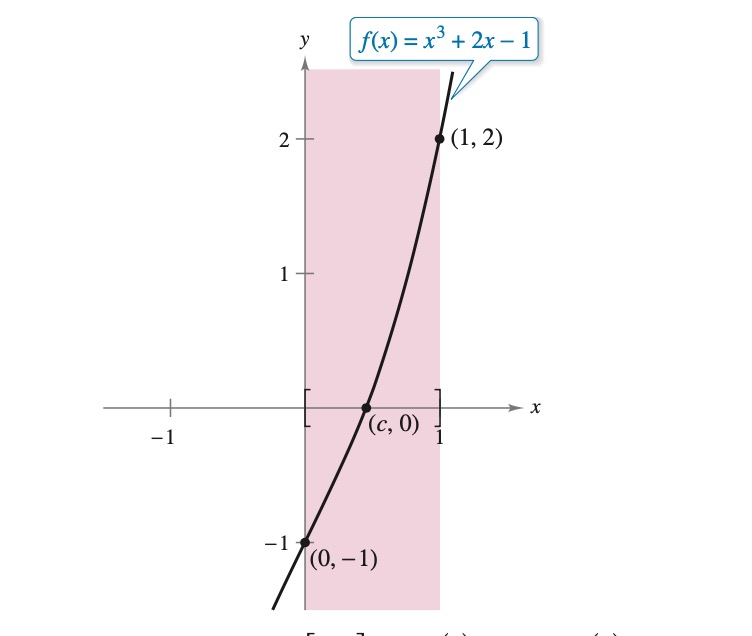
\includegraphics[width=0.600\linewidth]{Example_8.jpg} % Adjust the image width as necessary
    \captionof{figure}{}
    \label{fig:graph}
\end{minipage}
\end{tcolorbox}



\subsection{Infinite Limits}
\begin{Definition}{ Infinite Limits}{}
Let $f$ be a function that is defined at every real number in some open interval containing $c$ (except possibly at $c$ itself). The statement

\[
\lim_{x \to c} f(x) = \infty
\]


\end{Definition}

\begin{tcolorbox}[colback=examplebg, colframe=red!75!black, title=\textbf{EXAMPLE 1: Determining Infinite Limits from a Graph}, fonttitle=\bfseries, sharp corners]
Determine the limit of each function shown in Figure 6 as $x$ approaches 1 from the left and from the right.

\begin{minipage}{\linewidth}
    \centering
    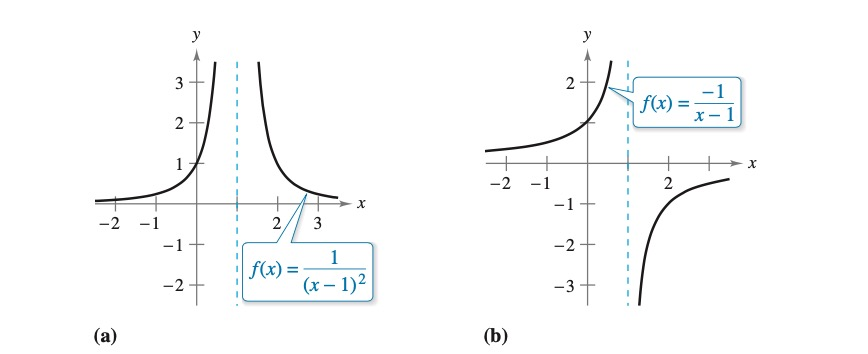
\includegraphics[width=0.560\linewidth]{Example_9.jpg} % Adjust the image width as necessary
    \captionof{figure}{}
    \label{fig:graph}
\end{minipage}

Each graph has an asymptote at $x = 1$. 
\tcblower
\subsection*{Solution:}

\textbf{a.} When $x$ approaches 1 from the left or the right, $(x - 1)^2$ is a small positive number. Thus, the quotient $1/(x - 1)^2$ is a large positive number, and $f(x)$ approaches infinity from each side of $x = 1$. So, you can conclude that
\[
\lim_{x \to 1} \frac{1}{(x - 1)^2} = \infty.
\]
Figure 1.41(a) confirms this analysis.

\textbf{b.} When $x$ approaches 1 from the left, $x - 1$ is a small negative number. Thus, the quotient $-1/(x - 1)$ is a large positive number, and $f(x)$ approaches infinity from the left of $x = 1$. So, you can conclude that
\[
\lim_{x \to 1^-} \frac{-1}{x - 1} = \infty.
\]

When $x$ approaches 1 from the right, $x - 1$ is a small positive number. Thus, the quotient $-1/(x - 1)$ is a large negative number, and $f(x)$ approaches negative infinity from the right of $x = 1$. So, you can conclude that
\[
\lim_{x \to 1^+} \frac{-1}{x - 1} = -\infty.
\]
\end{tcolorbox}
\subsubsection{Vertical Asymptotes}
\begin{Definition}{Vertical Asymptote}{}
If $f(x)$ approaches infinity (or negative infinity) as $x$ approaches $c$ from the right or the left, then the line $x = c$ is a \textbf{vertical asymptote} of the graph of $f$.
\end{Definition}

In Example 1, note that each of the functions is a quotient and that the vertical asymptote occurs at a number at which the denominator is 0 (and the numerator is not 0). 

\begin{mytheorem}{Vertical Asymptotes}{}

Let $f$ and $g$ be continuous on an open interval containing $c$. If $f(c) \neq 0$, $g(c) = 0$, and there exists an open interval containing $c$ such that $g(x) \neq 0$ for all $x \neq c$ in the interval, then the graph of the function
\[
h(x) = \frac{f(x)}{g(x)}
\]
has a vertical asymptote at $x = c$.


\end{mytheorem}

\begin{tcolorbox}[colback=examplebg, colframe=red!75!black, title=\textbf{EXAMPLE 2: A Rational Function with Common Factors}, fonttitle=\bfseries, sharp corners]
Determine all vertical asymptotes of the graph of 
\[
f(x) = \frac{x^2 + 2x - 8}{x^2 - 4}.
\]
\tcblower
\textbf{Solution:}
Begin by simplifying the expression, as shown:
\[
f(x) = \frac{x^2 + 2x - 8}{x^2 - 4} = \frac{(x + 4)(x - 2)}{(x + 2)(x - 2)} = \frac{x + 4}{x + 2}, \quad x \neq 2.
\]

At all $x$-values other than $x = 2$, the graph of $f$ coincides with the graph of 
\[
g(x) = \frac{x + 4}{x + 2}.
\]
So, you can apply Theorem 1.41 to $g$ to conclude that there is a vertical asymptote at $x = -2$. From the graph, you can see that
\[
\lim_{x \to -2^-} \frac{x^2 + 2x - 8}{x^2 - 4} = -\infty \quad \text{and} \quad \lim_{x \to -2^+} \frac{x^2 + 2x - 8}{x^2 - 4} = \infty.
\]

Note that $x = 2$ is \textbf{not} a vertical asymptote.
\end{tcolorbox}


\begin{mytheorem}{Properties of Infinite Limits}{}

Let $c$ and $L$ be real numbers, and let $f$ and $g$ be functions such that
\[
\lim_{x \to c} f(x) = \infty \quad \text{and} \quad \lim_{x \to c} g(x) = L.
\]

\begin{enumerate}
    \item \textbf{Sum or difference:} 
    \[
    \lim_{x \to c} [f(x) \pm g(x)] = \infty.
    \]

    \item \textbf{Product:} 
    \[
    \lim_{x \to c} [f(x)g(x)] = \infty, \quad L > 0,
    \]
    \[
    \lim_{x \to c} [f(x)g(x)] = -\infty, \quad L < 0.
    \]

    \item \textbf{Quotient:} 
    \[
    \lim_{x \to c} \frac{g(x)}{f(x)} = 0.
    \]
\end{enumerate}


\end{mytheorem}
\begin{tcolorbox}[colback=examplebg, colframe=red!75!black, title=\textbf{EXAMPLE 3: Determining Limits}, fonttitle=\bfseries, sharp corners]

\begin{enumerate}

    \item[\textbf{a.}] Because 
    \[
    \lim_{x \to 1} \left( x^2 + 1 \right) = 2 \quad \text{and} \quad \lim_{x \to 1^-} \cot (\pi x) = -\infty,
    \]
    you can write
    \[
    \lim_{x \to 1^-} \frac{x^2 + 1}{\cot (\pi x)} = 0. \quad \text{(Property 3, Theorem 1.4.2)}
    \]

    \item[\textbf{b.}] Because 
    \[
    \lim_{x \to 0^+} 3 = 3 \quad \text{and} \quad \lim_{x \to 0^+} \cot x = \infty,
    \]
    you can write
    \[
    \lim_{x \to 0^+} 3 \cot x = \infty. \quad \text{(Property 2, Theorem 1.4.2)}
    \]

    \item[\textbf{c.}] Because 
    \[
    \lim_{x \to 0} x^2 = 0 \quad \text{and} \quad \lim_{x \to 0} \frac{1}{x} = \infty,
    \]
    you can write
    \[
    \lim_{x \to 0} \left( \frac{x^2 + 1}{x} \right) = \infty. \quad \text{(Property 1, Theorem 1.4.2)}
    \]
\end{enumerate}
\end{tcolorbox}

\end{document}